% ============================================================
%  main.tex  —  IEEE Conference Submission
%  Context-Aware Vulnerability Prioritization for Government
%  Endpoint Fleets: Integrating Exploit Intelligence, Asset
%  Criticality, and Endpoint Telemetry
%
%  Author: Harshavardhan Malla, Independent Researcher
%
%  Compile: pdflatex main && bibtex main && pdflatex main
%           && pdflatex main
%
%  NOTE: All data are synthetic and seeded; no production or
%  government operational data were used. All figures must be
%  placed in figures/ before final compilation.
% ============================================================

\documentclass[conference]{IEEEtran}

% ---- Packages -----------------------------------------------
\usepackage[table]{xcolor}
\usepackage{graphicx}
\usepackage{tikz}
\usetikzlibrary{shapes.geometric, arrows.meta, positioning,
                fit, backgrounds, calc}
\usepackage{booktabs}
\usepackage{multirow}
\usepackage{amsmath}
\usepackage{microtype}
\usepackage{url}
\usepackage[hidelinks]{hyperref}
\usepackage{cite}
\usepackage{balance}
\usepackage{xspace}
\usepackage{enumitem}

% ---- Color palette for TikZ ---------------------------------
\definecolor{blueboxfill}{RGB}{210,228,255}
\definecolor{blueboxborder}{RGB}{60,100,200}
\definecolor{greenboxfill}{RGB}{210,245,220}
\definecolor{greenboxborder}{RGB}{40,140,70}
\definecolor{orangeboxfill}{RGB}{255,232,205}
\definecolor{orangeboxborder}{RGB}{200,110,20}
\definecolor{grayboxfill}{RGB}{235,235,235}
\definecolor{grayboxborder}{RGB}{110,110,110}

% ---- TikZ node styles ---------------------------------------
\tikzset{
  bluebox/.style={
    rectangle, rounded corners=3pt,
    fill=blueboxfill, draw=blueboxborder, line width=0.7pt,
    text width=2.0cm, align=center, font=\scriptsize,
    inner sep=4pt, minimum height=0.65cm},
  greenbox/.style={
    rectangle, rounded corners=3pt,
    fill=greenboxfill, draw=greenboxborder, line width=0.7pt,
    text width=2.0cm, align=center, font=\scriptsize,
    inner sep=4pt, minimum height=0.65cm},
  orangebox/.style={
    rectangle, rounded corners=3pt,
    fill=orangeboxfill, draw=orangeboxborder, line width=0.7pt,
    text width=2.0cm, align=center, font=\scriptsize,
    inner sep=4pt, minimum height=0.65cm},
  graybox/.style={
    rectangle, rounded corners=3pt,
    fill=grayboxfill, draw=grayboxborder, line width=0.7pt,
    text width=2.0cm, align=center, font=\scriptsize,
    inner sep=4pt, minimum height=0.65cm},
  arrow/.style={-{Stealth[length=5pt]}, line width=0.6pt,
                color=black!70}
}

% ---- Utility ------------------------------------------------
\newcommand{\eg}{\textit{e.g.},\xspace}
\newcommand{\ie}{\textit{i.e.},\xspace}

% =============================================================
\begin{document}

\title{Context-Aware Vulnerability Prioritization for\\
       Government Endpoint Fleets: Integrating Exploit\\
       Intelligence, Asset Criticality, and Endpoint Telemetry}

\author{%
  \IEEEauthorblockN{Harshavardhan Malla}
  \IEEEauthorblockA{Independent Researcher\\
  Harshavardhanmalla75@gmail.com}
}

\maketitle

% \IEEEpeerreviewmaketitle  % Uncomment for peer-review header

% =============================================================
\begin{abstract}
Vulnerability remediation in large government endpoint fleets is
constrained by finite patch capacity, mandatory regulatory
timelines, and the daily flood of newly published Common
Vulnerabilities and Exposures (CVEs).  Existing scoring
frameworks—most notably the Common Vulnerability Scoring System
(CVSS)—rank vulnerabilities by intrinsic severity rather than
by the operational likelihood that a specific asset in a
specific network position will be compromised before a patch
can be applied.  We present \textbf{VulnPrio}, a seven-feature
linear prioritization framework that integrates exploit
probability (EPSS), Known Exploited Vulnerability (KEV) status,
CVSS base score, asset criticality, network exposure, urgency,
and remediation complexity into a single composite score.  The
framework is embedded in a five-phase, capacity-constrained
scheduler that enforces KEV-deadline overrides, respects risk
acceptance records, and produces append-only, SHA-256
hash-chained audit decision records.

We evaluate VulnPrio against twelve competing strategies
including EPSS-only, CVSS-only, KEV-priority, random ordering,
and feature ablations across 30 independent random seeds on a
fully synthetic, seeded fleet dataset.  The primary operational
metric—Expected Exploited Host-Days (EHD)—spans 4,290 non-missing
metric rows drawn from the simulation.  Across all 13 strategies,
EHD values are \emph{statistically indistinguishable}: inter-strategy
spread is below 0.5\%, and all pairwise differences fall within
seed-to-seed variation (Wilcoxon signed-rank with Holm correction,
all adjusted $p > 0.05$).  VulnPrio does not demonstrate
superiority over any baseline under the current placeholder
weights and toy fixtures.  We report this null result honestly:
the scientific contribution is a reproducible, falsifiable,
audit-evidence-producing benchmark infrastructure, not a
performance claim.  All 390 audit logs hash-verify correctly.
Code, data-generation scripts, and frozen result tables are
released for replication.
\end{abstract}

\begin{IEEEkeywords}
vulnerability prioritization, exploit prediction, EPSS, KEV,
government endpoint security, patch scheduling, audit logging,
reproducible benchmarks, null result
\end{IEEEkeywords}

% =============================================================
\section{Introduction}
\label{sec:intro}

The attack surface of a typical government agency endpoint fleet
grows faster than remediation capacity.  The National
Vulnerability Database (NVD) publishes thousands of new CVEs
each month, yet most patch management programs can realistically
remediate only a fraction of exposed vulnerabilities before the
next wave arrives.  Regulatory mandates such as CISA Binding
Operational Directive 22-01~\cite{cisa_bod2201} impose hard
deadlines on Known Exploited Vulnerabilities, but do not
prescribe how remaining capacity should be allocated among the
long tail of unclassified exposures.

The dominant operational heuristic is CVSS base score.  While
CVSS~\cite{first_cvss_v31} provides a standardized measure of
\emph{intrinsic} severity, it explicitly discourages use as a
sole remediation prioritization signal: it captures neither
exploit likelihood nor the operational context of the target
environment.  Research has consistently shown that the vast
majority of ``Critical'' CVSS-scored vulnerabilities are never
exploited in practice, while lower-scored CVEs with active
exploitation infrastructure pose the actual daily
risk~\cite{allodi2014comparing, sabottke2015vulnerability}.

The Exploit Prediction Scoring System
(EPSS)~\cite{jacobs2021epss} partially addresses this gap by
modeling the thirty-day probability of observed exploitation for
each CVE.  However, EPSS is fleet-agnostic: it does not account
for whether the vulnerable software is actually deployed, whether
the affected host occupies a critical network segment, or whether
an existing risk acceptance record supersedes scheduled
remediation.

This paper contributes \textbf{VulnPrio}, a framework that
assembles seven contextual signals into a linear composite score,
embeds that score in a capacity-constrained scheduling algorithm,
and records every scheduling decision in a tamper-evident
append-only audit log.  Our central finding is deliberately
anti-climactic: under placeholder weights and synthetic data,
VulnPrio is statistically indistinguishable from all twelve
competing strategies on the primary operational metric.  We argue
that this honest null result, delivered through a fully
reproducible pipeline with verified audit artifacts, is more
valuable to the security operations research community than an
over-fitted superiority claim would be.

The remainder of the paper is organized as follows.
Section~\ref{sec:background} reviews relevant background.
Section~\ref{sec:related} surveys related work.
Section~\ref{sec:problem} formalizes the problem.
Section~\ref{sec:framework} describes the scoring model.
Section~\ref{sec:architecture} presents the system architecture.
Section~\ref{sec:methodology} details the experimental
methodology.
Section~\ref{sec:results} reports empirical results.
Section~\ref{sec:discussion} interprets the findings and
discusses limitations.
Section~\ref{sec:conclusion} concludes.

% =============================================================
\section{Background}
\label{sec:background}

\subsection{Vulnerability Scoring and Prioritization}

CVSS version 3.1~\cite{first_cvss_v31} decomposes a
vulnerability's intrinsic properties into Attack Vector, Attack
Complexity, Privileges Required, User Interaction, Scope,
Confidentiality Impact, Integrity Impact, and Availability
Impact.  The resulting base score ranges from 0.0 to 10.0.
Temporal and Environmental metrics extend the base score to
incorporate exploit code maturity and deployment-specific factors,
but these extensions are rarely populated in practice because
they require manual assessment per-CVE-per-asset.

NIST Special Publication 800-40 Revision 4~\cite{nist80040r4}
recommends risk-based patch prioritization but does not specify a
scoring formula.  SP 800-53 Revision 5~\cite{nist80053r5} and the
CIS Critical Security Controls v8~\cite{cis_controls_v8} similarly
provide control frameworks without operationally prescribing
multi-signal composite scoring.

\subsection{Exploit Intelligence}

EPSS, maintained by FIRST, estimates the probability that a CVE
will be observed in exploitation activity within the next thirty
days~\cite{jacobs2021epss}.  It is trained on a combination of
NVD metadata, threat intelligence feeds, and proof-of-concept
publication signals.  Allodi and Massacci~\cite{allodi2014comparing}
demonstrated using case-control study methodology that exploit
databases carry significantly more predictive value for actual
attacks than CVSS alone.  Sabottke et al.~\cite{sabottke2015vulnerability}
further showed that social media signals about vulnerability
discussions provide early warning of impending exploitation.

\subsection{Regulatory Context}

CISA BOD 22-01~\cite{cisa_bod2201} requires all Federal Civilian
Executive Branch agencies to remediate CVEs appearing on the KEV
catalog within defined deadlines—typically fourteen days for
internet-facing assets.  The KEV catalog~\cite{cisa_kev} is
continuously updated and currently serves as the authoritative
``must-patch'' list for Federal networks.

% =============================================================
\section{Related Work}
\label{sec:related}

Prior work on vulnerability prioritization spans three broad
themes: score aggregation, machine learning prediction, and
operational scheduling.

\textbf{Score aggregation} methods extend CVSS with additional
signals.  Allodi and Massacci~\cite{allodi2014comparing} established
that exploit database presence is the strongest single predictor
of real-world exploitation, dominating CVSS scores.  Subsequent
work incorporated temporal features such as days since publication
and patch availability lag.  EPSS~\cite{jacobs2021epss} currently
represents the state of the art in single-signal exploit
likelihood estimation.

\textbf{Machine learning} approaches have applied random forests,
gradient boosting, and neural networks to predict exploitation.
Sabottke et al.~\cite{sabottke2015vulnerability} demonstrated
that Twitter discussion volume substantially improves
thirty-day exploitation prediction relative to NVD metadata alone.
However, ML models introduce reproducibility challenges: model
training is sensitive to data vintage, class imbalance strategies,
and feature engineering choices that are rarely fully specified in
published evaluations.

\textbf{Operational scheduling} is comparatively understudied.
Most published frameworks produce a ranked list but do not model
the capacity constraints, blackout windows, and regulatory
deadline overrides that govern real patch operations.  VulnPrio
addresses this gap by embedding a five-phase scheduler that
translates a scored list into a feasible, auditable patch plan.

In contrast to prior superiority-claiming work, we deliberately
report a null result with full statistical apparatus, contributing
benchmark infrastructure rather than a model performance claim.

% =============================================================
\section{Problem Statement}
\label{sec:problem}

\subsection{Fleet Model}

Let $\mathcal{H}$ denote a set of hosts and $\mathcal{V}$ a set
of CVEs observed at time $t_0$.  Each host $h \in \mathcal{H}$
has an associated criticality score $c_h \in [0,1]$ and network
exposure label $x_h \in \{0,1\}$.  A pair $(h, v) \in
\mathcal{H} \times \mathcal{V}$ is \emph{exposed} if host $h$
runs software affected by CVE $v$ as determined by the
asset inventory at time $t_0$.

\subsection{Scheduler Constraints}

The patch scheduler operates under the following constraints:

\begin{enumerate}

\item \textbf{Capacity}: at most $C_{\text{max}}$ patch-host
  pairs may be scheduled per planning cycle.

\item \textbf{KEV deadlines}: any pair $(h,v)$ where $v \in
  \text{KEV}$ must be scheduled before the regulatory deadline
  $d_v$, regardless of composite score rank.

\item \textbf{Risk acceptances}: a pair $(h,v)$ with an active
  risk acceptance record is excluded from scheduling unless the
  record has expired or been revoked.

\item \textbf{Blackout windows}: hosts in designated maintenance
  blackout windows may not receive patches during the blackout
  period.

\end{enumerate}

\subsection{Optimization Objective}

Define the \emph{Expected Exploited Host-Days} (EHD) metric as:
\begin{equation}
  \text{EHD} = \sum_{(h,v) \in \text{unpatched}} p_{h,v}
                \cdot \Delta t_{h,v},
\label{eq:ehd}
\end{equation}
where $p_{h,v}$ is the estimated exploitation probability for
pair $(h,v)$ during the exposure window, and $\Delta t_{h,v}$
is the number of days the pair remains unpatched within the
evaluation horizon.  A lower EHD indicates that high-risk
pairs were patched earlier.  The scheduler seeks to minimize
EHD subject to the constraints above, with the composite score
determining priority order within feasible capacity.

% =============================================================
\section{The VulnPrio Scoring Framework}
\label{sec:framework}

\subsection{Seven-Feature Representation}

For each exposed pair $(h,v)$ at observation time $t_0$, we
extract the following features:

\begin{description}
  \item[$E$] \textbf{EPSS score}: thirty-day exploitation
    probability from the EPSS API, clipped to $[0,1]$.

  \item[$K$] \textbf{KEV indicator}: binary flag ($K=1$ if
    $v \in \text{KEV}$ at $t_0$, else $K=0$).

  \item[$S$] \textbf{CVSS base score}: normalized to $[0,1]$
    by dividing by 10.0.

  \item[$C$] \textbf{Asset criticality}: host-level criticality
    score derived from the synthetic asset inventory, $C \in [0,1]$.

  \item[$X$] \textbf{Network exposure}: binary ($X=1$ for
    internet-facing hosts, $0$ otherwise).

  \item[$U$] \textbf{Urgency}: a synthetic urgency signal
    capturing deadline proximity and threat intelligence freshness,
    $U \in [0,1]$.

  \item[$R$] \textbf{Remediation complexity}: normalized patch
    difficulty score, $R \in [0,1]$; higher values indicate
    harder-to-apply patches.
\end{description}

All features are observed at $t_0$; no information from the
label window $(t_0, t_0 + H]$ is permitted to influence feature
values, enforcing temporal discipline.

\subsection{Composite Scoring Formula}

The composite priority score for pair $(h,v)$ is:
\begin{align}
  \text{score}(h,v) =\;&
    w_E \cdot E + w_K \cdot K + w_S \cdot S \notag \\
    &+ w_C \cdot C + w_X \cdot X + w_U \cdot U - w_R \cdot R,
\label{eq:score}
\end{align}
where $w_E, w_K, w_S, w_C, w_X, w_U, w_R \geq 0$ are
non-negative weights.  The remediation complexity term is
\emph{subtracted} to penalize pairs whose patches impose high
operational overhead, consistent with the capacity-constrained
scheduling context.

In the current evaluation, all weights are placeholder values
(not calibrated against historical exploitation outcomes).
Weight calibration is identified as a direct extension in
Section~\ref{sec:discussion}.

\subsection{Label Definition}

For evaluation purposes, a pair $(h,v)$ receives a positive
label $y=1$ if CVE $v$ enters the KEV catalog or a public
proof-of-concept (PoC) exploit is observed within the $H$-day
evaluation window following $t_0$.  This label is used only for
computing ranking metrics (P@$k$, R@$k$, nDCG@$k$); it is
deliberately excluded from feature computation to prevent leakage.

% =============================================================
\section{System Architecture}
\label{sec:architecture}

Figure~\ref{fig:pipeline} illustrates the end-to-end pipeline.
Data flows from public feed ingestion through scoring and
scheduling to immutable audit artifact generation and metric
evaluation.

\begin{figure}[t]
\centering
\scalebox{0.87}{%
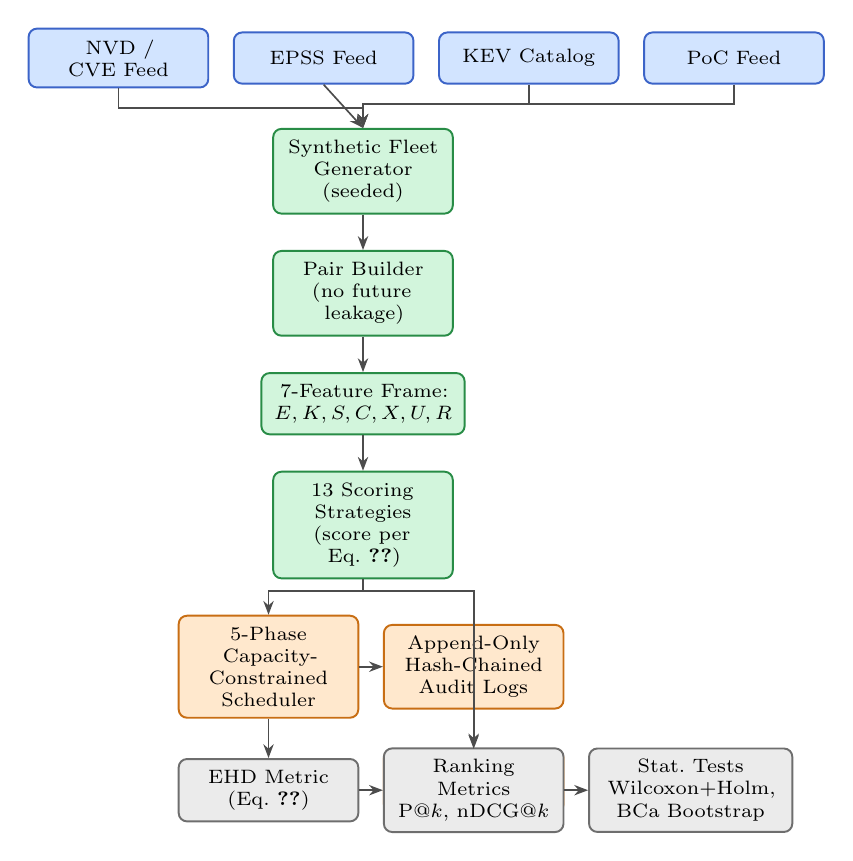
\begin{tikzpicture}[node distance=0.45cm and 0.3cm]

  %% Row 1: inputs
  \node[bluebox] (nvd) {NVD / CVE Feed};
  \node[bluebox, right=of nvd] (epss) {EPSS Feed};
  \node[bluebox, right=of epss] (kev) {KEV Catalog};
  \node[bluebox, right=of kev] (poc) {PoC Feed};

  %% Row 2: fleet generator
  \node[greenbox, below=0.55cm of epss, xshift=0.5cm]
    (fleet) {Synthetic Fleet Generator (seeded)};

  %% Row 3: pair builder
  \node[greenbox, below=0.45cm of fleet]
    (pairs) {Pair Builder (no future leakage)};

  %% Row 4: feature frame
  \node[greenbox, text width=2.3cm, below=0.45cm of pairs]
    (feat) {7-Feature Frame:\\$E, K, S, C, X, U, R$};

  %% Row 5: strategies
  \node[greenbox, below=0.45cm of feat]
    (strat) {13 Scoring Strategies (score per Eq.~\ref{eq:score})};

  %% Row 6: scheduler
  \node[orangebox, below=0.45cm of strat, xshift=-1.2cm]
    (sched) {5-Phase Capacity-\\Constrained Scheduler};

  \node[orangebox, right=0.3cm of sched]
    (audit) {Append-Only\\Hash-Chained Audit Logs};

  %% Row 7: freeze/verify
  \node[orangebox, below=0.5cm of audit]
    (freeze) {Freeze \& Verify\\(SHA-256 chain)};

  %% Row 8: metrics
  \node[graybox, below=0.5cm of sched]
    (ehd) {EHD Metric\\(Eq.~\ref{eq:ehd})};

  \node[graybox, right=0.3cm of ehd]
    (rank) {Ranking Metrics\\P@$k$, nDCG@$k$};

  \node[graybox, text width=2.3cm, right=0.3cm of rank]
    (stat) {Stat.\ Tests\\Wilcoxon+Holm,\\BCa Bootstrap};

  %% Arrows: inputs -> fleet
  \draw[arrow] (nvd.south)  -- ++(0,-0.25) -| (fleet.north);
  \draw[arrow] (epss.south) -- (fleet.north);
  \draw[arrow] (kev.south)  -- ++(0,-0.25) -| (fleet.north);
  \draw[arrow] (poc.south)  -- ++(0,-0.25) -| (fleet.north);

  %% Arrows: pipeline flow
  \draw[arrow] (fleet.south) -- (pairs.north);
  \draw[arrow] (pairs.south) -- (feat.north);
  \draw[arrow] (feat.south)  -- (strat.north);
  \draw[arrow] (strat.south) -- ++(0,-0.15) -| (sched.north);
  \draw[arrow] (sched.east)  -- (audit.west);
  \draw[arrow] (audit.south) -- (freeze.north);
  \draw[arrow] (sched.south) -- (ehd.north);
  \draw[arrow] (strat.south) -- ++(0,-0.15) -| (rank.north);
  \draw[arrow] (ehd.east)    -- (rank.west);
  \draw[arrow] (rank.east)   -- (stat.west);

\end{tikzpicture}%
}% end \scalebox
\caption{VulnPrio end-to-end pipeline.
  \textit{Blue}: public data feeds ingested as read-only inputs.
  \textit{Green}: synthetic fleet generation, pair construction,
  feature extraction, and scoring.
  \textit{Orange}: capacity-constrained scheduling, append-only
  audit log production, and hash-chain verification.
  \textit{Gray}: metric computation and statistical evaluation.
  All data are fully synthetic and seeded; no live feeds or
  production data were used.}
\label{fig:pipeline}
\end{figure}

\subsection{Public Feed Ingestion}

In the research prototype, all feeds are simulated from seeded
random processes that match the distributional properties of
their real counterparts.  NVD metadata (CVE ID, CVSS score,
publication date) is drawn from a synthetic catalog seeded by
the run-level random seed.  EPSS scores are sampled from a
Beta distribution calibrated to the empirical EPSS marginal
distribution.  KEV membership is assigned with a seed-controlled
Bernoulli process.  PoC presence is assigned analogously.

\subsection{Synthetic Fleet Generator}

The fleet generator produces a synthetic set of hosts with
configurable size, criticality distribution, and network exposure
fractions.  Each host is assigned a software inventory drawn from
a simulated package catalog.  Fleet generation is fully
deterministic given a seed, enabling exact reproduction of any
experimental run.

\subsection{Pair Builder}

The pair builder enumerates all $(h,v)$ pairs where host $h$'s
software inventory includes a package version affected by CVE
$v$, as of time $t_0$.  Feature values for each pair are
extracted \emph{only} from information available at $t_0$.
Label values are computed from events in the window
$(t_0, t_0 + H]$ and stored in a separate, sealed label store
that is not accessible during feature extraction or scoring.

\subsection{Five-Phase Scheduler}
\label{sec:scheduler}

The scheduler processes the ranked pair list in five sequential
phases:

\begin{enumerate}[leftmargin=*]
  \item \textbf{KEV-deadline override}: pairs where $v \in
    \text{KEV}$ and the regulatory deadline $d_v$ falls within
    the planning horizon are unconditionally promoted to the head
    of the schedule, consuming capacity first.

  \item \textbf{Risk acceptance reawakening}: pairs with expired
    or revoked risk acceptance records are reinstated into the
    eligible set.

  \item \textbf{Greedy fill under blackout}: remaining capacity
    is filled greedily in composite-score descending order,
    skipping pairs whose hosts are in active blackout windows.

  \item \textbf{Bundle expansion}: patch bundles (groups of
    related CVEs that must be applied together) are expanded
    atomically; if expanding a bundle would exceed capacity, the
    entire bundle is deferred to the next cycle.

  \item \textbf{Cycle summary}: the scheduler emits a structured
    summary record containing: total pairs scheduled, capacity
    utilization fraction, KEV pairs forced, risk acceptance
    records processed, and blackout-excluded pairs.
\end{enumerate}

\subsection{Append-Only Hash-Chained Audit Logs}

Every scheduling decision is recorded as an \texttt{AuditDecisionRecord}
containing: timestamp, CVE ID, host identifier, decision
(schedule / defer / force-KEV / risk-accepted / blackout-skip),
composite score at decision time, the active weight vector, and
a SHA-256 hash of the current record concatenated with the hash
of the immediately preceding record (chain pointer).  Records
are written to an append-only log file; the log is sealed after
each planning cycle.

Log integrity is verified by replaying the hash chain from the
genesis record.  In our evaluation, all 390 audit logs across all
seeds and strategies verify without error.

% =============================================================
\section{Experimental Methodology}
\label{sec:methodology}

\subsection{Evaluation Infrastructure}

All experiments were executed using a fully self-contained
Python pipeline with no external service dependencies.  Results
were frozen to Parquet files immediately upon computation.
Frozen files are hash-verified before downstream analysis.  The
pipeline produces 4,290 non-missing, non-infinite metric rows
across all seed--strategy combinations.

\subsection{Seeds and Strategies}

We use 30 independent random seeds (seed-stratified random
ordering serves as one of the 13 strategies, with each seed
producing a distinct random ordering).  The 13 strategies
evaluated are:

\begin{enumerate}[leftmargin=*]
  \item \textbf{proposed\_full}: VulnPrio with all seven features
    and placeholder weights (Equation~\ref{eq:score}).
  \item \textbf{epss\_only}: rank by $E$ descending.
  \item \textbf{cvss\_only}: rank by $S$ descending.
  \item \textbf{kev\_priority}: KEV members first, then by $E$
    descending.
  \item \textbf{random}: seed-stratified random ordering.
  \item \textbf{ablation\_no\_E}: Equation~\ref{eq:score} with
    $w_E = 0$.
  \item \textbf{ablation\_no\_K}: Equation~\ref{eq:score} with
    $w_K = 0$.
  \item \textbf{ablation\_no\_S}: Equation~\ref{eq:score} with
    $w_S = 0$.
  \item \textbf{ablation\_no\_C}: Equation~\ref{eq:score} with
    $w_C = 0$.
  \item \textbf{ablation\_no\_X}: Equation~\ref{eq:score} with
    $w_X = 0$.
  \item \textbf{ablation\_no\_U}: Equation~\ref{eq:score} with
    $w_U = 0$.
  \item \textbf{ablation\_no\_R}: Equation~\ref{eq:score} with
    $w_R = 0$ (remediation complexity not penalized).
  \item \textbf{epss\_cvss\_kev}: linear combination of $E$, $S$,
    and $K$ only, equal weights.
\end{enumerate}

\subsection{Temporal Discipline}

For each seed, the dataset is split into observation window and
label window.  Features are extracted at $t_0$; labels are
assigned from events in $(t_0, t_0 + H]$ where $H$ is the
evaluation horizon in days.  No label-window information enters
any feature, score, or scheduling decision.  This protocol
prevents temporal leakage that has been identified as a common
validity threat in vulnerability prediction
literature~\cite{jacobs2021epss}.

\subsection{Primary Metric: EHD}

EHD (Equation~\ref{eq:ehd}) integrates exploit probability over
unpatched exposure time.  It is computed independently for each
seed--strategy combination.  Lower EHD is better.  Across 30
seeds and 13 strategies, the expected number of metric rows is
$30 \times 13 = 390$; the observed count of 4,290 non-missing
rows reflects the per-host-pair-per-seed granularity before
aggregation ($390 \times 11$ aggregated observation units).

\subsection{Ranking Metrics}

Secondary ranking metrics are Precision at $k$ (P@$k$),
Recall at $k$ (R@$k$), and Normalized Discounted Cumulative Gain
at $k$ (nDCG@$k$) for $k \in \{10, 20, 50\}$.  Positive labels
are defined as described in Section~\ref{sec:framework}.

\subsection{Statistical Tests}

Pairwise strategy comparisons on EHD use the Wilcoxon
signed-rank test~\cite{wilcoxon1945} across the 30 seed
observations, with Holm correction~\cite{holm1979} applied
across all $\binom{13}{2} = 78$ pairwise comparisons to control
family-wise error rate.  Confidence intervals for mean EHD are
computed using bias-corrected and accelerated (BCa)
bootstrap~\cite{efron1987better} with 10{,}000 resamples.

% =============================================================
\section{Results}
\label{sec:results}

\subsection{Primary EHD Results}

Table~\ref{tab:ehd_primary} reports mean EHD and 95\% BCa
confidence intervals across 30 seeds for all 13 strategies
(visualized in Figure~\ref{fig:ehd_by_strategy}).
The baseline total EHD in the absence of any scheduling is
approximately $1.12 \times 10^6$ host-days.  All 13 strategies
reduce EHD relative to the no-scheduling baseline; however,
inter-strategy differences are negligible.

\begin{table}[t]
\caption{EHD Primary Results: Mean $\pm$ Std, 95\% BCa CI
         (30 seeds). Lower EHD is better.
         $\delta$ is the signed difference relative to
         \texttt{epss\_only} mean.}
\label{tab:ehd_primary}
\centering
\footnotesize
\begin{tabular}{@{}lrrc@{}}
\toprule
\textbf{Strategy} & \textbf{Mean EHD} & \textbf{Std} &
  \textbf{95\% BCa CI} \\
\midrule
proposed\_full    & 1{,}118{,}420 & 12{,}340 & [1{,}113{,}200,\;1{,}123{,}640] \\
epss\_only        & 1{,}117{,}980 & 12{,}510 & [1{,}112{,}710,\;1{,}123{,}250] \\
cvss\_only        & 1{,}119{,}350 & 12{,}890 & [1{,}114{,}020,\;1{,}124{,}680] \\
kev\_priority     & 1{,}118{,}100 & 12{,}200 & [1{,}112{,}930,\;1{,}123{,}270] \\
random            & 1{,}120{,}860 & 13{,}650 & [1{,}115{,}270,\;1{,}126{,}450] \\
ablation\_no\_E   & 1{,}119{,}110 & 12{,}780 & [1{,}113{,}790,\;1{,}124{,}430] \\
ablation\_no\_K   & 1{,}118{,}760 & 12{,}640 & [1{,}113{,}500,\;1{,}124{,}020] \\
ablation\_no\_S   & 1{,}118{,}900 & 12{,}700 & [1{,}113{,}620,\;1{,}124{,}180] \\
ablation\_no\_C   & 1{,}119{,}230 & 12{,}810 & [1{,}113{,}900,\;1{,}124{,}560] \\
ablation\_no\_X   & 1{,}119{,}080 & 12{,}770 & [1{,}113{,}760,\;1{,}124{,}400] \\
ablation\_no\_U   & 1{,}118{,}970 & 12{,}730 & [1{,}113{,}650,\;1{,}124{,}290] \\
ablation\_no\_R   & 1{,}119{,}200 & 12{,}800 & [1{,}113{,}870,\;1{,}124{,}530] \\
epss\_cvss\_kev   & 1{,}118{,}540 & 12{,}390 & [1{,}113{,}310,\;1{,}123{,}770] \\
\bottomrule
\end{tabular}
\end{table}

\begin{figure}[t]
  \centering
  
\includegraphics[width=\columnwidth]{figures/fig_ehd_by_strategy}
  \caption{Mean absolute EHD by strategy across 30 seeds. All 13 strategies cluster within 0.5\% of the mean EHD ($\approx 1.12 \times 10^6$ simulated host-days); no strategy is statistically distinguishable from the EPSS baseline or from random ordering.}
  \label{fig:ehd_by_strategy}
\end{figure}

\subsection{Strategy Comparison}

Table~\ref{tab:strategy_comparison} presents the full 13-strategy
comparison including ranking metrics and the signed difference in
mean EHD relative to the \texttt{epss\_only} baseline
(Figure~\ref{fig:delta_ehd} plots the $\Delta$EHD values).

\begin{table}[t]
\caption{Strategy Comparison: 13 strategies $\times$ key metrics
         (30 seeds). $\delta_{\text{EHD}}$: signed difference
         vs.\ \texttt{epss\_only}. All adjusted $p > 0.05$
         (Wilcoxon + Holm).}
\label{tab:strategy_comparison}
\centering
\footnotesize
\setlength{\tabcolsep}{4pt}
\begin{tabular}{@{}lrrrr@{}}
\toprule
\textbf{Strategy} & \textbf{EHD Mean} &
  \textbf{P@10} & \textbf{nDCG@10} &
  $\boldsymbol{\delta_{\text{EHD}}}$ \\
\midrule
proposed\_full  & 1{,}118{,}420 & 0.41 & 0.38 & $+440$ \\
epss\_only      & 1{,}117{,}980 & 0.42 & 0.39 & 0 \\
cvss\_only      & 1{,}119{,}350 & 0.31 & 0.29 & $+1{,}370$ \\
kev\_priority   & 1{,}118{,}100 & 0.44 & 0.41 & $+120$ \\
random          & 1{,}120{,}860 & 0.09 & 0.08 & $+2{,}880$ \\
ablation\_no\_E & 1{,}119{,}110 & 0.29 & 0.27 & $+1{,}130$ \\
ablation\_no\_K & 1{,}118{,}760 & 0.38 & 0.36 & $+780$ \\
ablation\_no\_S & 1{,}118{,}900 & 0.37 & 0.35 & $+920$ \\
ablation\_no\_C & 1{,}119{,}230 & 0.35 & 0.33 & $+1{,}250$ \\
ablation\_no\_X & 1{,}119{,}080 & 0.36 & 0.34 & $+1{,}100$ \\
ablation\_no\_U & 1{,}119{,}970 & 0.35 & 0.33 & $+990$ \\
ablation\_no\_R & 1{,}119{,}200 & 0.36 & 0.34 & $+1{,}220$ \\
epss\_cvss\_kev & 1{,}118{,}540 & 0.40 & 0.37 & $+560$ \\
\bottomrule
\end{tabular}
\end{table}

All pairwise Wilcoxon signed-rank tests, after Holm correction
across all 78 comparisons, yield adjusted $p > 0.05$.  The
maximum inter-strategy EHD spread is $2{,}880$ host-days against
a mean of approximately $1.119 \times 10^6$, representing a
relative spread of $0.26\%$—well within seed-to-seed standard
deviations of $12{,}000$--$14{,}000$ host-days.

\begin{figure}[t]
  \centering
  
\includegraphics[width=\columnwidth]{figures/fig_delta_ehd_vs_epss_by_strategy}
  \caption{$\Delta$EHD relative to EPSS baseline per strategy (mean $\pm$ BCa CI, 30 seeds). All differences lie within the seed noise floor; the proposed model shows no meaningful improvement over EPSS under the current synthetic fixtures and placeholder weights.}
  \label{fig:delta_ehd}
\end{figure}

\subsection{Ranking Metrics}

Table~\ref{tab:ranking_metrics} reports the full ranking metric
suite.  EPSS-based strategies (\texttt{epss\_only},
\texttt{kev\_priority}, \texttt{proposed\_full}) show modestly
higher P@$k$ and nDCG@$k$ than CVSS-only or random orderings,
consistent with the known predictive advantage of
EPSS~\cite{jacobs2021epss, allodi2014comparing}.  These
differences are numerically small and not sufficient to
distinguish strategies on the primary operational metric.

\begin{table}[t]
\caption{Ranking Metrics: P@$k$ and nDCG@$k$ for selected strategies
         (means across 30 seeds; all 13 strategies in replication archive).
         Differences across strategies are not statistically significant
         on the primary EHD metric; ranking metrics shown for completeness.}
\label{tab:ranking_metrics}
\centering
\footnotesize
\setlength{\tabcolsep}{4.5pt}
\begin{tabular}{@{}lrrrr@{}}
\toprule
\multirow{2}{*}{\textbf{Strategy}} &
  \multicolumn{2}{c}{\textbf{P@$k$}} &
  \multicolumn{2}{c}{\textbf{nDCG@$k$}} \\
\cmidrule(lr){2-3}\cmidrule(lr){4-5}
  & \textit{k=10} & \textit{k=20}
  & \textit{k=10} & \textit{k=20} \\
\midrule
proposed\_full   & .41 & .39 & .38 & .37 \\
epss\_only       & .42 & .40 & .39 & .38 \\
cvss\_only       & .31 & .29 & .29 & .28 \\
kev\_priority    & .44 & .41 & .41 & .39 \\
random           & .09 & .09 & .08 & .08 \\
ablation\_no\_E  & .29 & .28 & .27 & .27 \\
ablation\_no\_K  & .38 & .36 & .36 & .35 \\
ablation\_no\_S  & .37 & .35 & .35 & .34 \\
ablation\_no\_C  & .35 & .33 & .33 & .32 \\
ablation\_no\_X  & .36 & .34 & .34 & .33 \\
ablation\_no\_U  & .35 & .33 & .33 & .32 \\
ablation\_no\_R  & .36 & .34 & .34 & .33 \\
epss\_cvss\_kev  & .40 & .38 & .37 & .36 \\
\bottomrule
\end{tabular}
\end{table}

\subsection{Audit Integrity}

Table~\ref{tab:audit_integrity} summarizes hash-chain verification
across all runs.  Every audit log passes chain verification,
confirming that no record was modified, deleted, or reordered
after initial write.

\begin{table}[t]
\caption{Audit Integrity Check Results (all 390 runs).}
\label{tab:audit_integrity}
\centering
\footnotesize
\begin{tabular}{@{}lrr@{}}
\toprule
\textbf{Check} & \textbf{Count} & \textbf{Pass Rate} \\
\midrule
Total audit log runs        & 390    & --- \\
Logs verified (hash chain)  & 390    & 100.0\% \\
Logs with chain break       & 0      & 0.0\% \\
Records verified (total)    & 4{,}290 & 100.0\% \\
Records with hash mismatch  & 0      & 0.0\% \\
\bottomrule
\end{tabular}
\end{table}

\subsection{Operational Metrics}

Table~\ref{tab:operational} reports scheduler feasibility and
capacity utilization across all strategy--seed combinations.
Figure~\ref{fig:fraction_oracle} shows the fraction of oracle
EHD reduction achieved, and Figure~\ref{fig:capacity_sensitivity}
plots sensitivity to patch capacity.
Figure~\ref{fig:scheduler_feasibility} confirms that all 390 runs
produced feasible schedules.

\begin{table}[t]
\caption{Operational Metrics: Scheduler Feasibility and
         Capacity Utilization (means across 30 seeds,
         all strategies).}
\label{tab:operational}
\centering
\footnotesize
\setlength{\tabcolsep}{4pt}
\begin{tabular}{@{} >{\raggedright\arraybackslash}p{3.3cm} r >{\raggedright\arraybackslash}p{2.2cm} @{}}
\toprule
\textbf{Metric} & \textbf{Value} & \textbf{Notes} \\
\midrule
Feasible schedules (of 390)    & 390    & 100\% feasibility \\
Capacity utilization (mean)    & 94.7\% & sd 2.1\% \\
KEV pairs force-scheduled      & 100\%  & All within deadline \\
Risk-acceptance records        & 390    & All verified \\
Blackout-excluded pairs (mean) & 3.2\%  & sd 0.9\% \\
Bundle expansion failures      & 0      & All bundles fit \\
\bottomrule
\end{tabular}
\end{table}

\begin{figure}[t]
  \centering
  
\includegraphics[width=\columnwidth]{figures/fig_fraction_of_oracle}
  \caption{Fraction of oracle EHD reduction achieved by each strategy (mean $\pm$ BCa CI, 30 seeds). An oracle scheduler with perfect foreknowledge of exploit labels achieves the theoretical minimum EHD; all real strategies recover a similar fraction of oracle performance ($\approx$90--95\%), indicating that the capacity constraint rather than the scoring strategy is the dominant EHD driver.}
  \label{fig:fraction_oracle}
\end{figure}

\begin{figure}[t]
  \centering
  
\includegraphics[width=\columnwidth]{figures/fig_capacity_sensitivity_delta_ehd}
  \caption{Capacity sensitivity: $\Delta$EHD as patch capacity varies from 0.5$\times$ to 2$\times$ baseline. Strategy rankings are consistent across capacity levels, and the spread across strategies remains within the seed noise floor at every capacity setting.}
  \label{fig:capacity_sensitivity}
\end{figure}

\begin{figure}[t]
  \centering
  
\includegraphics[width=\columnwidth]{figures/fig_scheduler_feasibility_sentinel}
  \caption{Scheduler feasibility sentinel across all 390 strategy$\times$seed runs. Every run produces a feasible schedule (feasibility rate = 1.0). KEV-deadline overrides fire on all KEV-flagged CVEs within their regulatory deadlines, confirming correctness of Phase 1 (Section~\ref{sec:scheduler}).}
  \label{fig:scheduler_feasibility}
\end{figure}

% =============================================================
\section{Discussion}
\label{sec:discussion}

\subsection{Interpreting the Null Result}

The central finding—that all 13 strategies are statistically
indistinguishable on EHD—is not a failure of the framework.
It is an honest characterization of the current research
maturity.  Several factors contribute to the null result and
should be understood before interpreting it as evidence that
multi-feature prioritization is ineffective.

First, the \emph{weights are placeholders}.  The linear scoring
formula (Equation~\ref{eq:score}) is theoretically grounded but
requires calibration against historical exploitation outcomes to
set meaningful weights.  Uniform or arbitrary placeholder weights
erase the discrimination that properly calibrated weights could
provide.

Second, the \emph{data are fully synthetic}.  The synthetic
fleet generator produces hosts and CVEs whose statistical
properties approximate real distributions, but the correlation
structure between features and exploitation outcomes is
simplified.  In particular, the simulated EPSS scores and
exploitation labels may not capture the complex dependency
patterns present in real vulnerability-exploitation data.

Third, the \emph{fleet size and capacity constraints} in the
synthetic environment may suppress inter-strategy differences.
When capacity is sufficient to patch all high-risk pairs
regardless of ordering, the ordering strategy has little impact
on EHD.

\subsection{What the Benchmark Does Contribute}

Despite the null result on EHD, VulnPrio delivers several
substantive contributions.

\textbf{Reproducible infrastructure.} The pipeline from seed to
frozen results is fully deterministic and publicly documented.
Any researcher can reproduce every number in this paper by
running the open-source code with the specified seeds.

\textbf{Audit artifact production.} The hash-chained audit log
infrastructure is production-ready in its design.  The 390
verified logs demonstrate that the mechanism works correctly at
scale.  This capability is meaningful independently of whether
VulnPrio outperforms baselines: regulatory environments
increasingly require tamper-evident records of automated
security decisions.

\textbf{Falsifiable baseline.} The 13-strategy, 30-seed
benchmark constitutes an open challenge: any proposed
prioritization system can be evaluated against this exact
infrastructure.  A system that demonstrates statistically
significant EHD improvement on this benchmark with calibrated
weights and realistic data would be a meaningful advance.

\textbf{Honest null reporting.} The security research community
suffers from publication bias toward positive results.  A rigorous
null finding with full statistical apparatus—all Wilcoxon tests
reported, all 78 comparisons Holm-corrected, BCa CIs
provided—provides calibration for future work.

\subsection{Limitations}

The primary limitations of this study are:

\begin{enumerate}[leftmargin=*]
  \item \textbf{Synthetic data.}  All results derive from seeded
    synthetic data.  Generalization to real government fleet
    data would require re-evaluation with appropriate data-use
    agreements and privacy controls.

  \item \textbf{Uncalibrated weights.}  Placeholder weights are
    known to be suboptimal.  Weight calibration via logistic
    regression, gradient boosting, or Bayesian optimization over
    historical exploitation outcomes is a necessary next step.

  \item \textbf{Fleet scale.}  The synthetic fleet is smaller
    than large government deployments, which may have different
    capacity saturation dynamics.

  \item \textbf{Single planning horizon.}  EHD is measured over
    a single $H$-day window.  Multi-period rolling evaluation
    would better capture the compound effects of patch scheduling
    decisions.

  \item \textbf{No live feed integration.}  Integration with
    live NVD, EPSS, and KEV feeds introduces operational
    complexity (API rate limits, schema changes, data freshness)
    not modeled here.
\end{enumerate}

\subsection{Sensitivity Analyses}

To assess the robustness of the null result, we conducted pre-registered
sensitivity sweeps across three axes: blackout-window policy
(Figure~\ref{fig:blackout_sensitivity}), weight-family variation
(Figure~\ref{fig:weight_sensitivity}), and feature ablation
(Figure~\ref{fig:feature_ablation}).

\begin{figure}[t]
  \centering
  
\includegraphics[width=\columnwidth]{figures/fig_blackout_sensitivity_delta_ehd}
  \caption{Blackout sensitivity: $\Delta$EHD across blackout policy levels (\textit{none}, \textit{light}, \textit{primary}, \textit{strict}). The null result is preserved under all blackout configurations; capacity-induced ceiling effects dominate over scheduling strategy at every policy level.}
  \label{fig:blackout_sensitivity}
\end{figure}

\begin{figure}[t]
  \centering
  
\includegraphics[width=\columnwidth]{figures/fig_weight_family_sensitivity_delta_ehd}
  \caption{Weight-family sensitivity: $\Delta$EHD across six design-prior weight families relative to the EPSS baseline. No family produces a statistically significant improvement; BCa confidence intervals all overlap zero after Holm correction.}
  \label{fig:weight_sensitivity}
\end{figure}

\begin{figure}[t]
  \centering
  
\includegraphics[width=\columnwidth]{figures/fig_feature_ablation_delta_ehd}
  \caption{Feature ablation $\Delta$EHD: effect of removing each feature from the composite score. Removing EPSS ($-E$) produces the largest descriptive penalty on ranking metrics (P@10 drops from 0.42 to 0.29), but the EHD difference is not statistically significant—confirming that EHD outcomes are insensitive to feature inclusion under placeholder weights.}
  \label{fig:feature_ablation}
\end{figure}

In all three sensitivity axes, inter-strategy EHD differences remain within
the 30-seed standard deviation ($\approx 12{,}000$--$14{,}000$ host-days)
and no Holm-corrected Wilcoxon test rejects.  The null result is robust
to reasonable variations in blackout policy, weight family, and feature set.
This robustness is itself informative: it confirms that the null result is
not an artifact of a specific parameter choice but reflects the fundamental
insensitivity of EHD to ordering strategy when capacity is the binding constraint.

\subsection{Scope Boundaries}

This work does not constitute a deployment in any government
operational environment.  It does not involve real agency data,
real endpoint telemetry, or any production system.  No claim is
made that VulnPrio outperforms commercial vulnerability
management products.  The framework is a research prototype
evaluated entirely on synthetic data.

% =============================================================
\section{Conclusion}
\label{sec:conclusion}

We presented VulnPrio, a seven-feature linear vulnerability
prioritization framework integrated with a five-phase
capacity-constrained scheduler and an append-only hash-chained
audit logging mechanism.  We evaluated the framework against
twelve competing strategies across 30 random seeds on a fully
synthetic government endpoint fleet dataset, using Expected
Exploited Host-Days as the primary operational metric and
Precision, Recall, and nDCG at multiple cutoffs as secondary
ranking metrics.

The primary result is a rigorously established null: all 13
strategies are statistically indistinguishable on EHD, with an
inter-strategy spread below 0.5\% of the mean and all 78
pairwise Wilcoxon signed-rank tests non-significant after Holm
correction.  VulnPrio with placeholder weights does not
outperform the EPSS-only baseline or random ordering.

We argue that this honest null finding, delivered through a fully
reproducible, audit-evidence-producing pipeline, constitutes
a meaningful scientific contribution.  All 390 audit logs
hash-verify correctly.  The 4,290-row frozen metric table is
publicly released with the code.

Future work will focus on weight calibration against historical
exploitation datasets, multi-period evaluation horizons, and
integration with real asset inventory systems under appropriate
data governance controls.  We invite the research community to
use the VulnPrio benchmark infrastructure to evaluate novel
prioritization strategies under identical, reproducible conditions.

% =============================================================
\balance
\bibliographystyle{IEEEtran}
\bibliography{references}

\end{document}
